% Template created by Jon Hood

\documentclass[letterpaper, 10pt, twoside]{article}
\usepackage{noto}
\usepackage{fancyhdr}
\usepackage{graphicx}
\usepackage{multirow}
\usepackage[table]{xcolor}
\usepackage[breaklinks=true]{hyperref}
\usepackage[letterpaper, top=1in, bottom=1in, left=1.5in, right=1in, includeheadfoot]{geometry}
\usepackage{wrapfig}
\usepackage{attachfile}
\usepackage{luatex85}
\usepackage{tikz}
\usetikzlibrary{shapes,arrows,positioning}

%                Main Variables
\newcommand{\repdate}{\formatdate{4}{5}{2020}}
\def \ProjectName{Security Technical Implementation Guide Qt Viewer}
\def \ProjectAcronym{STIGQter}
\def \ProjectVersion{1.0.1}

%-------------------------------------------------------------------------------
%                Header & Footer Setup
%-------------------------------------------------------------------------------
\pagestyle{fancy}
\lhead[\thepage]{
\includegraphics[height = 2em]{images/STIGQter.pdf}}
\chead{\ProjectName\ --- \ProjectVersion}
\rhead[{
\includegraphics[height = 2em]{images/STIGQter.pdf}}]{\thepage}
\cfoot{\ProjectAcronym\ \ProjectVersion}

\fancypagestyle{blank}
{
	\lhead{}
	\chead{}
	\rhead{}
	\cfoot{}
	\lfoot{}
}

%-------------------------------------------------------------------------------
%                Revisions Table
%-------------------------------------------------------------------------------
\definecolor{STIGQterBlue}{RGB}{30,72,124}
\newcounter{RevisionCounter}
\newenvironment{Revision}{
	\begin{center}
		\begin{tabular}{ | c | c | c | p{23em} | }
			\hline
			\multicolumn{4}{| c |}{\cellcolor{STIGQterBlue}\textbf{\textcolor{white}{Revision History}}} \\
			\hline
			\rowcolor{lightgray}
			\textbf{Date} & \textbf{Revision} & \textbf{Revised By} & \textbf{Reason} \\
			\hline
		}{
	\end{tabular}
\end{center}
}
\newcommand{\RevisionEntry}[3]{\stepcounter{RevisionCounter}
	#1 & \Alph{RevisionCounter} & #2 & #3 \\
	\hline}

%-------------------------------------------------------------------------------
%                Title Page
%-------------------------------------------------------------------------------
\newcommand{\headerlogo}{
	
\includegraphics[width=.3\linewidth]{images/STIGQter.pdf}\\
	\vspace{.5em}
}
\newcommand{\docline}{\textmd{\textbf{STIGQter Configuration, Installation, and Usage Guide\\}}}
\newcommand{\generator}{Generated By: Jon Hood}
\title{
	\headerlogo
	\docline
	\vspace{.5em}
	\normalsize{\generator}
}

\author{Jon Hood}
\date{\repdate}

%-------------------------------------------------------------------------------
%                PDF metadata
%-------------------------------------------------------------------------------
\hypersetup
{
	pdfauthor= (Jon Hood),
	pdftitle =  (STIGQter Installation and Usage Guide)
}

\usepackage{attachfile}
\usepackage[backend=biber]{biblatex}
\usepackage{import}
\usepackage{graphicx}
\usepackage[utf8]{inputenc}
\usepackage{url}
\addbibresource{sources.bib}
\usepackage{setspace}
\usepackage{array}
\usepackage{booktabs}
\newcolumntype{L}{@{}>{\kern\tabcolsep}l<{\kern\tabcolsep}}
\usepackage{colortbl}
\usepackage{xcolor}
\usepackage{textcomp}
\usepackage{outlines}
\usepackage{setspace}
\usepackage{longtable}
\usepackage{enumitem}
\usepackage{listings}
\usepackage{pgfplots}
\usepgfplotslibrary{fillbetween}
\usepackage{datetime}
\newdateformat{changelog}{\THEMONTH/\THEDAY/\THEYEAR}

\lstdefinestyle{CStyle} {language=C}
\lstdefinestyle{CSharpStyle} {language=[Sharp]C}
\lstdefinestyle{PHPStyle} {language=php}
\lstdefinestyle{JavaStyle} {language=java}
\lstdefinestyle{BashStyle} {language=bash}

\lstset{language=C}
\lstset{language=[Sharp]C}
\lstset{language=php}
\lstset{language=java}
\lstset{language=bash}

\newcolumntype{L}[1]{>{\raggedright\let\newline\\\arraybackslash\hspace{0pt}}m{#1}}
\newcolumntype{C}[1]{>{\centering\let\newline\\\arraybackslash\hspace{0pt}}m{#1}}
\newcolumntype{R}[1]{>{\raggedleft\let\newline\\\arraybackslash\hspace{0pt}}m{#1}}

%start the document
\begin{document}

%generate a title page
\thispagestyle{blank}
\maketitle
\newpage

\thispagestyle{blank}
This page intentionally left blank for 2-sided printing compatibility.
\newpage

%tell the page counter to restart
\setcounter{page}{1}
\pagenumbering{roman} %use lowercase Roman numerals for page numbers

%Revision History page
\begin{Revision}
\RevisionEntry{\date{\changelog\formatdate{29}{10}{2019}}}{Jon Hood}{Initial Release of Documentation}
\RevisionEntry{\date{\changelog\formatdate{28}{1}{2020}}}{Jon Hood}{Prepare for 1.0 Release}
\RevisionEntry{\date{\changelog\formatdate{4}{5}{2020}}}{Jon Hood}{Prepare for 1.0.1 Release}
\end{Revision}
\newpage

%generate a table of contents
\setcounter{tocdepth}{2}
\tableofcontents
\cleardoublepage % go to next right-side page

%reset the page counter for the regular pages
\setcounter{page}{1}
\doublespacing
\pagenumbering{arabic} %use standard numbers for the page number

\section{Background}
STIGViewer has been the DISA-provided tool of choice for creating STIG Checklists (CKL) and Continuous Monitoring Risk Scoring (CMRS) reports for eMASS. It is a solid tool, stable, and unfortunately closed-source. STIGQter attempts to recreate the features of STIGViewer in an open and extensible way. The goal of STIGQter is to abide by free and open source principles so that it may be incorporated and distributed freely in any operating system.

\section{Starting Up}

STIGQter connects to \url{https://nvd.nist.gov/} and \url{https://dl.dod.cyber.mil/} (linked to from \url{https://public.cyber.mil/}).

\begin{figure}[h]
	\tikzstyle{block} = [rectangle, draw, fill=blue!20, text width=5em, text centered, rounded corners, minimum height=4em]
	\tikzstyle{extern} = [draw, ellipse,fill=red!20, node distance=3cm, minimum height=2em]
	\tikzstyle{line} = [draw, -latex']
	\begin{tikzpicture}
		\node [block] (STIGQter) {STIGQter Application};
		\node [extern, left of=STIGQter, xshift=-7em] (Cyber) {https://dl.dod.cyber.mil/};
		\node [extern, right of=STIGQter, xshift=7em] (NIST) {https://nvd.nist.gov/};
		\path [line] (STIGQter) -- node {Port: 443} (Cyber);
		\path [line] (STIGQter) -- node {Port: 443} (NIST);
	\end{tikzpicture}
	\caption{Data Flow Diagram}
	\label{fig:dataflow}
\end{figure}

To use STIGQter, you will need to index the set of RMF Controls from NIST, the set of CCIs from DISA, and obtain the relevant STIGs for your system. Figure~\ref{fig:dataflow} shows the data flow for the application.

\clearpage
\subsection{Indexing Controls and CCIs}
\begin{wrapfigure}{R}{0.6\textwidth}
	\centering
	\vspace{-10pt}
	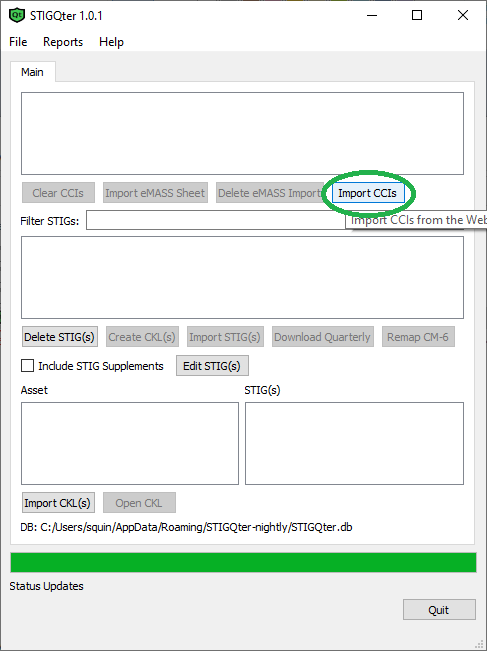
\includegraphics[width=0.59\textwidth]{images/main-01.png}
	\caption{Starting Main Interface}
	\vspace{-30pt}
	\label{fig:importccis}
\end{wrapfigure}


The first step in using STIGQter is to index the latest RMF Controls and CCIs from NIST and Cyber.mil respectively. To do this, click the ``Import CCIs'' button (Figure~\ref{fig:importccis}).

STIGQter will index the base CCIs associated with NIST 800-53 Revision 4 automatically. When done, it will download the latest CCI list from DISA to incorporate the latest DoD modifications. These CCIs form the base units of validation in eMASS: issues are recorded at the CCI level and roll up to the Control level.

\subsection{Indexing STIGs}

\begin{wrapfigure}{L}{0.6\textwidth}
	\centering
	\vspace{-10pt}
	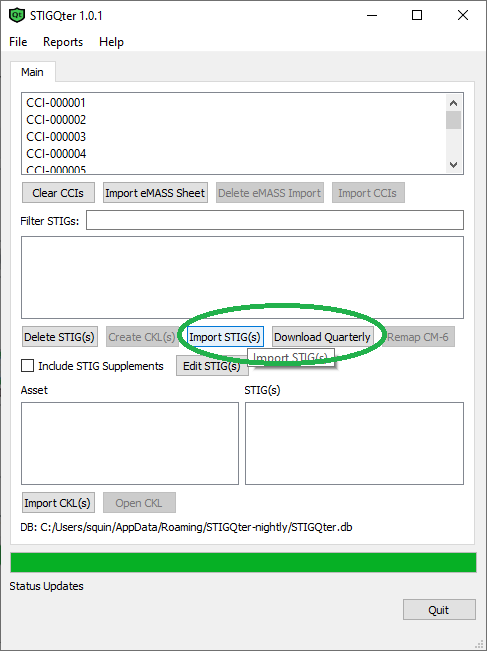
\includegraphics[width=0.59\textwidth]{images/main-02.png}
	\caption{Importing STIGs}
	\vspace{-40pt}
	\label{fig:importstigs}
\end{wrapfigure}
DISA generally publishes Security Technical Implementation Guides and Security Requirements Guides (STIG/SRG) at \url{http://public.cyber.mil/stigs/}. The ``document library'' provides a list of STIGs available for download. These STIG .zip files may be downloaded and imported into the application (Figure~\ref{fig:importstigs}). Beginning with version 1.0.1, the quarterly release from DISA can be downloaded and imported.

STIGs and SRGs provide a checklist of weaknesses and security problems in common environments. These checklists provide a bare minimum security posture for a system or component. Checklist items in each STIG and SRG are mapped to CCIs, and these CCIs map to controls in the NIST 800-53 Risk Management Framework (RMF) process.

When importing a STIG or SRG, these mappings may be incorrect. When a STIG check is mapped against a CCI that does not exist in 800-53rev4, a warning displays asking to file a bug report with DISA to fix this mapping. The check is then remapped against control CM-6 under CCI-366.

\paragraph{NOTE:} Checklists created from a STIG/SRG must match down to the version/release number.

\subsection{Importing Checklists}

Finally, existing checklist (CKL) files can be imported if their corresponding STIG/SRG is already imported. Note that the CKL format changed with STIGViewer version 2. It is impossible to automatically map the CKL file to its corresponding STIG checklist in CKLs created with STIGViewer 1.x.

Checklists can be created and viewed within STIGQter without having to import previous content as well. After selecting the applicable STIGs, the user may create a new Asset based on these STIGs. The primary view of editing checklist data is Asset-based. Each Asset has a set of STIGs mapped to it.

\section{Managing a Checklist/Asset}

Now that existing or new Asset(s) have been set up, the compliance status of their checks can be modified. Checklists in STIGQter are asset-based. A single asset can contain multiple STIGs and SRGs as part of its checklist.

\paragraph{Example:} Suppose that Foo is a Microsoft SQL Server-based web application. As a software engineer, you have been tasked with obtaining an RMF Assess Only approval for the Foo software and an ATO for your organization's implementation of Foo. In your organization's nonsensical Foo setup, the web server is running on Apache on a Windows XP system, and the Microsoft SQL Server 2018 instance is being emulated on Ubuntu 18.04.

\subsection{Asset Viewer}

The Asset can be viewed in a screen similar to the classic STIGViewer screen. STIGs can be added and removed from the Asset, and compliance status of each checklist item can be recorded.

Shortcuts for the compliance state of the selected checklist item(s) are:
\begin{itemize}
	\item CTRL+N: Not a Finding
	\item CTRL+O: Open Finding
	\item CTRL+R: Not Reviewed
	\item CTRL+X: Not Applicable
\end{itemize}

Marking checklist items as open findings will automatically adjust the compliance status of the generated reports. Open checklist findings cause their respective CCIs to become open, and open CCIs will cause their respective RMF Controls to become open.

When selecting new STIGs for an Asset, their checks are added to the database. When removing a checklist from a STIG, both the checks and the previous compliance information is removed from the database.

\section{Reports}

STIGQter provides several useful reports. These reports are meant to provide high-level summaries to management-level personnel, interface with other RMF systems, and give user-readable roll-up details to the user.

\subsection{eMASS Test Results}

eMASS is the system of choice for DoD RMF compliance data. When exporting and importing control-level data with eMASS, this is the recommended report to use.

\subsubsection{Importing eMASS Test Results}

When importing eMASS test results, STIGQter will pull in previous compliance information for the control including all documentation reviews that have been completed. This test result (TR) import is used as the baseline of controls for RMF compliance information. It is assumed that the system being imported into STIGQter has completed their CNSSI 1253 categorization, applied any applicable overlays, gone through all tailoring steps, and applied all inheritance relationships.

\paragraph{Limitations:} There are some meaningful limitations to the eMASS test result import:
\begin{itemize}
	\item The Assessment Procedure Acronym (AP Acronym) is ignored. In the past 2 years, these acronyms have been renumbered twice. It is highly recommended to ignore this field. Additionally, there is no fully unclassified source for AP Acronyms. These are maintained by the eMASS developers and are not standardized. If you write tools that rely on AP Acronyms, at some point in the future, it will break.
	\item CM-6 CCI-366 should not be inherited. STIGs that don't map to CCIs in the imported system's baseline are remapped to CCI-366. If this control is inherited, failed STIG results will not be recorded in eMASS even though they show up in STIGQter.
	\item Report classifications are not imported. STIGQter does not maintain the system's classification and leaves protection of the data up to the user.
\end{itemize}

\subsubsection{Exporting eMASS Test Results}

The eMASS TR Report can be exported so that it can then be re-imported into eMASS with the STIG compliance that has been recorded in STIGQter.

\paragraph{Limitations:}

The TR Report may not be in the same order as the one generated by eMASS. Filtering is automatically applied to be able to sort this sheet. Additionally, AP Acronyms are ignored and classification levels are not preserved.

\section{Editing STIGs}

Beginning in Version 1.0.1, limited STIG editing ability has been added. These features are considered "testing." Modifying STIGs may compromise their data and importability into other applications. Checklists created from modified STIGs may cause unexpected behavior in other systems.

\section{Export Formats}

STIGQter provides several different formats for interface with different systems.

\subsection{Internal STIGQter Format}

The STIGQter format is a SQLite database. It can be saved (compressed) and opened as a normal .stigqter file. You are encouraged to use a SQLite database browser to look through its structure, manipulate any mappings that are needed, and extend STIGQter. Note, however, that modifying the database can destroy the integrity of your data.

Beginning with STIGQter 1.0.0, reverse compatibility is maintained. When database formats change, the database is dynamically upgraded to the latest version supported by your STIGQter software. You are encouraged to save off the .stigqter file for reference at a later date if needed. There is no need to maintain the version of STIGQter used with the .stigqter file.

On Windows systems, the internal database is stored at \texttt{\%appdata\%\textbackslash\allowbreak STIGQter\textbackslash\allowbreak STIGQter.db}. On Linux and most other operating systems, the internal database is stored at \texttt{\textasciitilde /.local/\allowbreak share/\allowbreak STIGQter/\allowbreak STIGQter.db}. Only the user and administrators have access to this file. User and administrator roles and permissions are handled at the operating system level.

\subsection{CKL Checklists}

Two CKL checklist file types can be produced in STIGQter:

\begin{enumerate}
	\item A single-asset CKL file that stores all STIGs and SRGs assigned to the asset (accessible from the ``Save CKL'' button when viewing the asset)
	\item A large number of CKLs that each contain a single Asset and STIG combination (accessible from the ``STIG CKLs'' report from the Reports menu)
\end{enumerate}

\subsection{Continuous Monitoring Risk Scoring}

The CMRS report can be provided to eMASS' Asset Manager. Overridden scores and mappings are not supported in the CMRS format, so this export is only recommended when using CMRS files in the eMASS Asset Manager.

\section{RMF Compliance}

The following documentation is available for RMF compliance purposes (double-click to open the file):
\begin{itemize}
	\item \textattachfile[color=0 0 0]{ac.pdf}{Access Control}
	\item \textattachfile[color=0 0 0]{au.pdf}{Audit and Accountability}
	\item \textattachfile[color=0 0 0]{at.pdf}{Awareness and Training}
	\item \textattachfile[color=0 0 0]{cm.pdf}{Configuration Management}
	\item \textattachfile[color=0 0 0]{cp.pdf}{Contingency Planning}
	\item \textattachfile[color=0 0 0]{ia.pdf}{Identification and Authentication}
	\item \textattachfile[color=0 0 0]{ma.pdf}{Maintenance}
	\item \textattachfile[color=0 0 0]{mp.pdf}{Media Protection}
	\item \textattachfile[color=0 0 0]{pm.pdf}{Program Management}
	\item \textattachfile[color=0 0 0]{ca.pdf}{Security Assessment and Authorization}
	\item \textattachfile[color=0 0 0]{sc.pdf}{System and Communications Protection}
	\item \textattachfile[color=0 0 0]{si.pdf}{System and Information Integrity}
	\item \textattachfile[color=0 0 0]{sa.pdf}{System and Services Acquisition}
\end{itemize}

\clearpage
\printbibliography

\end{document}
